\documentclass[tikz,border=6pt]{standalone}
\usepackage{xcolor}
\definecolor{popvision}{HTML}{7aa2c4}
\definecolor{popodor}{HTML}{e0a04a}
\definecolor{popcontact}{HTML}{8d6b4a}
\definecolor{poploom}{HTML}{c45c4a}
\definecolor{popinter}{HTML}{e7e2da}
\definecolor{popmotor}{HTML}{16140f}
\begin{document}
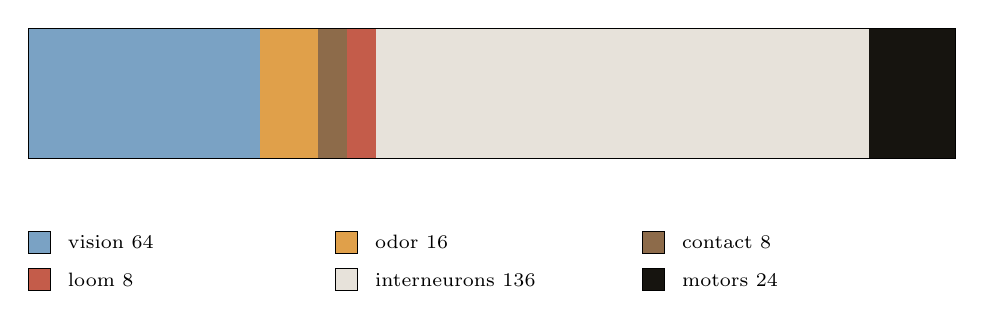
\begin{tikzpicture}
  \begin{scope}[x=0.046cm,y=0.046cm]
    \fill[popvision] (0,0) rectangle (64,36);
    \fill[popodor] (64,0) rectangle (80,36);
    \fill[popcontact] (80,0) rectangle (88,36);
    \fill[poploom] (88,0) rectangle (96,36);
    \fill[popinter] (96,0) rectangle (232,36);
    \fill[popmotor] (232,0) rectangle (256,36);
    \draw (0,0) rectangle (256,36);
  \end{scope}
  \foreach \col/\row/\name/\swatch in {0/0/{vision 64}/popvision, 1/0/{odor 16}/popodor, 2/0/{contact 8}/popcontact, 0/1/{loom 8}/poploom, 1/1/{interneurons 136}/popinter, 2/1/{motors 24}/popmotor} {
    \fill[\swatch] ({\col*3.9}, {-1.2-\row*0.48}) rectangle ({\col*3.9+0.28}, {-0.92-\row*0.48});
    \draw ({\col*3.9}, {-1.2-\row*0.48}) rectangle ({\col*3.9+0.28}, {-0.92-\row*0.48});
    \node[anchor=west,font=\scriptsize] at ({\col*3.9+0.38}, {-1.06-\row*0.48}) {\name};
  }
\end{tikzpicture}
\end{document}
